\chapter{From First-Principles Impurity Operators to Effective-Mass Models}
\index{impurity operator!model classes|textbf}

\label{app:impurity-model-classes}

\chapterstatus{synthesis with two human-accepted calculated synthetic
numerical-verification results and a proposed subsequent research program. The
spin-space and one-dimensional defect-extraction calculations remain within
bounded finite-model scopes.
The appendix does not claim an accepted production Kohn--Sham parent, Wannier
operator, aligned material impurity operator, fitted material lattice or
continuum model, crossover radius, calculated material binding energy, or
scientific validation result.}

\section{Physical objective}

The central objective is to determine when a finite operator extracted from a
first-principles semiconductor calculation can be replaced by a constrained
lattice or continuum model without losing the observables and operator
structure required for its intended use. The problem is not to establish a
universally exact effective Hamiltonian. It is to identify the least complex
admissible model class that reproduces a declared parent problem within
separately specified spectral, subspace, operator, and bound-state tolerances.

The parent description is a self-consistent Kohn--Sham calculation in the
Born--Oppenheimer fixed-ion framework~\cite{hohenberg1964,kohn1965}. In the
initial program, exchange and correlation are represented by the PBE
generalized-gradient approximation~\cite{perdew1996}, and the electron--ion
interaction is represented by compatible optimized norm-conserving Vanderbilt
pseudopotentials from the approved PseudoDojo family~\cite{hamann2013,vansetten2018}.
These choices define the
parent model against which later reductions are evaluated. Disagreement between
the parent calculation and experiment is not automatically a reduction error.

\citationtodo{medium priority}{Separate the Born--Oppenheimer attribution from
the DFT and Kohn--Sham attributions. Check the fixed-ion statement against Born
and Oppenheimer (1927), provisional key \texttt{bornOppenheimer1927}, and retain
\texttt{hohenberg1964} and \texttt{kohn1965} only
for the narrower claims they support.}

The Kohn--Sham band gap is likewise a property of the selected parent
approximation and is not identified with the exact quasiparticle gap. The
distinction between the Kohn--Sham eigenvalue gap and the fundamental gap is
established by the derivative-discontinuity analysis of exact
density-functional theory~\cite{perdewLevy1983,shamSchluter1983}.

\section{Representation hierarchy}

The proposed reduction is organized as the sequence
\begin{equation}
    \hat H_{\mathrm{KS},s}
    \longrightarrow
    \hat H_s^{(P)}
    \longrightarrow
    \mathbf H_{\mathrm W,s}^{(P)}
    \longrightarrow
    \Delta\mathbf H_{\mathrm W,d}^{(P)}
    \longrightarrow
    \hat H_{\mathrm{model},d},
\end{equation}
where $s=b$ denotes the pristine host and $s=d$ a doped system. The arrows
represent distinct operations:
\begin{enumerate}
    \item selection of a retained Kohn--Sham subspace;
    \item construction of a localized Wannier representation;
    \item alignment of pristine and doped retained spaces;
    \item construction of an impurity operator; and
    \item approximation within a restricted lattice or continuum model class.
\end{enumerate}

Projection, localization, alignment, truncation, and model fitting introduce
different assumptions and must remain separately auditable. Wannier
localization changes representation but does not by itself reduce matrix rank.
For entangled bands, the retained subspace must be selected before the gauge is
localized~\cite{marzari2012,souza2001}.

\section{Pristine silicon reference}

The host is crystalline silicon in the diamond structure. A reproducible
parent identity requires the lattice vectors, basis-site convention,
reciprocal-coordinate convention, pseudopotential files, plane-wave cutoff,
$k$-point mesh, occupation treatment, self-consistency thresholds, relaxation
criteria, spin treatment, spin--orbit setting, and producing-program version.

The initial bulk pilot targets a band-edge subspace suitable for comparison
with a constrained orthogonal $sp^3s^{\ast}$ Slater--Koster hierarchy. The
principal spectral observables are the indirect Kohn--Sham gap, the
conduction-valley position, and the longitudinal and transverse electron
effective masses. Withheld-point band errors are required to separate
interpolation or fitting performance from transferability outside the training
set.

Spectral agreement is necessary but not sufficient. Two Hamiltonians can
reproduce the same selected eigenvalues while differing substantially as
operators. The bulk compatibility study must therefore evaluate both spectral
observables and unitary-aligned operator residuals where a common operator
representation has been established. The least complex acceptable
tight-binding class is the first member of the declared hierarchy that
satisfies all required tolerances; additional parameters are not justified
solely because they further reduce the training error.

\citationtodo{medium priority}{Check the constrained orthogonal
$sp^3s^{\ast}$ silicon pilot and its Slater--Koster hierarchy against
Slater--Koster (1954) and Vogl et al. (1983), bibliography keys
\texttt{slater1954} and \texttt{vogl1983} (already present).}

\section{Aligned impurity operator}
\index{impurity operator!aligned}


Let
\begin{equation}
    \hat H_b^{(P)}:
    \mathcal H_b^{(P)}
    \longrightarrow
    \mathcal H_b^{(P)}
\end{equation}
and
\begin{equation}
    \hat H_d^{(P)}:
    \mathcal H_d^{(P)}
    \longrightarrow
    \mathcal H_d^{(P)}
\end{equation}
be the retained pristine and doped Hamiltonians. Their matrices cannot be
subtracted solely because they have equal dimensions. A unitary identification
\begin{equation}
    \hat U_d:
    \mathcal H_b^{(P)}
    \longrightarrow
    \mathcal H_d^{(P)}
\end{equation}
must be fixed using declared orbital, geometric, gauge, spin, and
energy-reference conventions. This appendix chooses the pristine retained space as the reference and defines
\begin{equation}
    \Delta\hat H_{d\rightarrow b}^{(P)}
    =
    \hat U_d^\dagger
    \hat H_d^{(P)}
    \hat U_d
    -
    \hat H_b^{(P)}.
\end{equation}
An equivalent convention transports the pristine operator to the doped space:
\begin{equation}
    \Delta\hat H_{b\rightarrow d}^{(P)}
    =
    \hat H_d^{(P)}
    -
    \hat U_d
    \hat H_b^{(P)}
    \hat U_d^\dagger
    =
    \hat U_d
    \Delta\hat H_{d\rightarrow b}^{(P)}
    \hat U_d^\dagger.
\end{equation}
The direction must remain explicit. In the remainder of this appendix,
$\Delta\hat H_d^{(P)}$ abbreviates the pristine-reference operator
$\Delta\hat H_{d\rightarrow b}^{(P)}$.

This operator is the primary first-principles difference object. It should not
be defined automatically as an impurity potential. It can contain local
electrostatic structure, nonlocal pseudopotential contributions, changes in the
self-consistent Hartree and exchange--correlation operators,
lattice-relaxation effects, intervalley and interorbital coupling, and
projection-induced nonlocality.

Equal total retained dimensions guarantee the existence of an abstract unitary
identification, but not a physically justified one. A momentum-preserving
identification additionally requires compatible retained dimensions in
corresponding Bloch fibers. In a localized representation, the alignment must
control site correspondence, orbital ordering, Wannier gauge, energy zero,
lattice geometry, and supercell mapping.

\section{Non-identifiability of an effective potential}
\index{identifiability!effective potential}


Let $\hat T_0^{(P)}$ be a declared kinetic reference on
$\mathcal H_b^{(P)}$. The difference
\begin{equation}
    \hat R_{T_0,d}^{(P)}
    =
    \Delta\hat H_d^{(P)}
    -
    \Delta\hat T_{0,d}^{(P)}
\end{equation}
is a reference-dependent residual operator. In the common case where the host
kinetic reference is assumed unchanged by the impurity model,
\begin{equation}
    \Delta\hat T_{0,d}^{(P)}=\hat 0,
\end{equation}
and the full aligned impurity operator is assigned to the residual. This
assignment remains a model convention rather than a deduction that the
operator is a local potential.

For any Hermitian operator $\hat K$ on the retained space,
\begin{equation}
    \Delta\hat H_d^{(P)}
    =
    \left(
        \Delta\hat T_{0,d}^{(P)}+\hat K
    \right)
    +
    \left(
        \hat R_{T_0,d}^{(P)}-\hat K
    \right).
\end{equation}
The aligned Hamiltonian difference alone does not uniquely determine a kinetic
correction and a potential correction. Their separation becomes identifiable
only after the kinetic structure and the admissible impurity-potential class
have been fixed.

\section{Admissible model classes}
\index{model class!impurity}


A native model class may act on a lattice, continuum, or other declared model
space $\mathcal X_m$. Let
\begin{equation}
    \mathcal M_{d,\mathrm{native}}^{(m)}
    =
    \left\{
        \Delta\hat K_d^{(m)}(\boldsymbol\theta):
        \mathcal X_m\longrightarrow\mathcal X_m
        \;\middle|\;
        \boldsymbol\theta\in\Theta_m
    \right\}.
\end{equation}
Before an operator norm is formed, each native candidate must be transported by
a declared model-to-reference map into
$\mathcal L(\mathcal H_b^{(P)})$. Denote the resulting represented candidate by
\begin{equation}
    \widetilde{\Delta\hat H}_d^{(m)}(\boldsymbol\theta):
    \mathcal H_b^{(P)}
    \longrightarrow
    \mathcal H_b^{(P)}.
\end{equation}
For a lattice class already expressed in the pristine reference coordinates,
the transport may be the identity. A useful declared hierarchy may include:
\begin{enumerate}
    \item a local isotropic screened-Coulomb potential;
    \item an anisotropic effective-mass potential;
    \item a multivalley local operator;
    \item a finite-range nonlocal lattice operator;
    \item orbital-block and neighbor-shell extensions; and
    \item an explicitly nonlocal static downfolded operator.
\end{enumerate}
These classes need not be nested merely because they appear in one list. Any
claim of least complexity requires a separately declared ordering and complete
acceptance rule. An energy-dependent downfolded operator
$\Delta\hat K_d^{(m)}(E;\boldsymbol\theta)$ requires an additional declared
energy domain and an energy-resolved operator, action, or resolvent comparison.
It is not governed by the static objective below merely by suppressing its
energy argument.

For an energy-independent class in a finite-dimensional identified
representation, suppose first that the minimum is attained and choose
\begin{equation}
    \boldsymbol\theta_{d,m}^{\star}
    \in
    \operatorname*{arg\,min}_{\boldsymbol\theta\in\Theta_m}
    \left\lVert
        \Delta\hat H_d^{(P)}
        -
        \widetilde{\Delta\hat H}_d^{(m)}(\boldsymbol\theta)
    \right\rVert_{\mathrm{HS}}^2.
\end{equation}
The corresponding minimum operator separation is
\begin{equation}
    d_d^{(m)}
    =
    \left\lVert
        \Delta\hat H_d^{(P)}
        -
        \widetilde{\Delta\hat H}_d^{(m)}
        (\boldsymbol\theta_{d,m}^{\star})
    \right\rVert_{\mathrm{HS}}.
\end{equation}
If the minimum is not known to be attained, the model-class separation should
instead be defined by the corresponding infimum over $\Theta_m$.

The quantity $d_d^{(m)}$ measures the expressiveness of the model class after
alignment. It is not merely an optimization diagnostic. If the minimum
separation remains above the prescribed tolerance, the model class is
structurally inadequate even when selected eigenvalues can be fitted.

An effective potential is therefore defined only relative to a declared class.
If $\mathcal M_V$ is a class of admissible potential operators and the minimum
is attained, then
\begin{equation}
    \hat V_{d,\mathcal M}^{\star}
    \in
    \operatorname*{arg\,min}_{\hat V\in\mathcal M_V}
    \left\lVert
        \hat R_{T_0,d}^{(P)}-\hat V
    \right\rVert_{\mathrm{HS}}^2.
\end{equation}
The raw residual $\hat R_{T_0,d}^{(P)}$ is not itself assigned the name
effective potential unless membership in, or approximation by, the declared
potential class has been established.

\section{Continuum effective-mass limit}
\index{effective-mass model!continuum limit}


Effective-mass and envelope-function theories derive continuum equations from
perturbed periodic systems~\cite{luttingerKohn1955,burt1992,burt1999}. Their
validity depends on retained-band structure, scale separation, valley content,
interface or impurity length scales, and the treatment of boundary conditions.
The effective Hamiltonian and admissible boundary conditions must be derived
consistently; incorrect symmetrization can produce nonphysical
solutions~\cite{foreman1993}. First-principles envelope-function constructions
demonstrate that a continuum operator can, in principle, be derived from an
atomistic parent rather than introduced solely by
phenomenology~\cite{foreman2005}.

Let
\begin{equation}
    \hat J_d:
    \mathcal H_{\mathrm{EMT},d}^{(P)}
    \longrightarrow
    \mathcal H_b^{(P)}
\end{equation}
identify a finite-dimensional discretization of the continuum envelope-function
space with a subspace of the pristine retained space. If $\hat J_d$ is an
isometric embedding, a parameterized continuum impurity operator can be tested
through
\begin{equation}
    \boldsymbol\theta_{\mathrm{EMT},d}^{\star}
    \in
    \operatorname*{arg\,min}_{\boldsymbol\theta\in\Theta_{\mathrm{EMT}}}
    \left\lVert
        \Delta\hat H_d^{(P)}
        -
        \hat J_d
        \Delta\hat H_{\mathrm{EMT},d}(\boldsymbol\theta)
        \hat J_d^\dagger
    \right\rVert_{\mathrm{HS}}^2,
\end{equation}
when the minimum is attained. This full-space loss treats the embedded
continuum operator as zero on the orthogonal complement of
$\operatorname{Ran}\hat J_d$ and assigns all complement and cross-block content
of the atomistic operator to the residual. If the intended comparison concerns
only the embedded continuum sector, both operands must instead be compressed by
$\hat P_J=\hat J_d\hat J_d^\dagger$. A non-isometric identification requires an
explicit metric, dual map, or generalized comparison rather than this formula
without qualification.

Recent multivalley analysis of Si/SiGe systems shows that an exact
valley-sector reduction can produce band-limited envelopes and nonlocal
potential operators, particularly when atomically sharp structure invalidates
a conventional slowly varying local approximation~\cite{ermoneit2026}; the
source equations and their project-specific limits are extracted in
Appendix~\ref{app:envelope-theory}. This provides a direct precedent for treating
locality as a model-class hypothesis.

The atomistic-to-continuum crossover should consequently be expressed as a
scale-dependent validation statement. A proposed crossover radius $r_{c,d}$
may be defined as the smallest tested radius beyond which both the declared
exterior residual and the declared interior--exterior cross-coupling residual
remain within their separate tolerances. Such a definition separates the
existence of a long-range
continuum regime from the unresolved short-range central-cell operator. If no
tested radius passes, the result should remain explicitly unresolved or be
recorded as no finite crossover over the tested domain.

\section{Dopant branches and validation}
\index{validation!dopant}


For substitutional phosphorus, the neutral $\mathrm P_{\mathrm{Si}}^0$
supercell contains both the donor-core perturbation and an additional valence
electron. The primary branch is scalar relativistic, collinearly spin
polarized, and non-SOC so that the odd electron count is represented. The
resulting neutral calculation must not be silently reinterpreted
as an isolated ionized donor. Each finite supercell describes a periodic dopant
array, so isolated-donor claims require supercell-size and shape convergence.

For substitutional boron, the neutral $\mathrm B_{\mathrm{Si}}^0$ supercell has
one fewer valence electron than the matched pristine cell. Final acceptor and
valence-manifold claims require a matching fully relativistic, noncollinear
spinor treatment with spin--orbit coupling. Scalar-relativistic calculations
may remain useful for method development but
must be labeled as a restricted branch.

Charged-defect corrections and dilute-limit interpretations require their own
controlled assumptions and convergence evidence~\cite{freysoldt2009,freysoldt2014}.
These issues belong to the parent and finite-size validation layers and should
not be absorbed into an operator-fitting residual without diagnosis.

\citationtodo{medium priority}{Check the phosphorus donor, boron acceptor,
spin--orbit valence-manifold, and periodic-supercell qualifications against the
appropriate donor/envelope, semiconductor, and defect-supercell sources.
Candidate existing keys: \texttt{luttingerKohn1955}, \texttt{yuCardona2010}, and
\texttt{freysoldt2014}.}

The principal validation quantities should remain distinct:
\begin{itemize}
    \item the global aligned operator error $\varepsilon_{H,d}$;
    \item the retained-subspace or projector error $\varepsilon_{\Pi,d}$;
    \item the binding-energy error $\Delta E_{b,d}$;
    \item the wavefunction or subspace fidelity $F_d$; and
    \item the continuum crossover radius $r_{c,d}$.
\end{itemize}
No single metric certifies the reduction. Spectral agreement does not imply
operator agreement, a small global norm can conceal a localized central-cell
failure, and a correct binding energy does not establish the transferability of
the underlying impurity operator.

\section{Proposed warmup program}

The impurity-reduction chain should be exercised first on controlled models in
which the relevant state-space maps and defect operators are known. The
spin-space and one-dimensional exercises below are human accepted; later stages
remain proposed work. Their purpose is to verify the mathematical construction
and separate failure modes before a first-principles silicon impurity operator
is interpreted.

Three headline warmups organize the program: comparison of spinless and
spinful state spaces, extraction from matched one-dimensional pristine and
defect supercells, and the corresponding extraction in two dimensions. Each
headline warmup requires the folding, null, planted-defect, alignment,
finite-size, model-class, and observable controls described below.

\subsection{Warmup 1: Spinless, spin-degenerate, collinear, and spinor spaces}

Let $\mathcal V$ be a finite orbital space and let
\begin{equation}
    \mathbf H_0:\mathcal V\longrightarrow\mathcal V
\end{equation}
be a spinless Hamiltonian. A nonmagnetic spinful lift acts on
$\mathcal V\otimes\mathbb C^2$:
\begin{equation}
    \mathbf H_{\mathrm{deg}}
    =
    \mathbf H_0\otimes\mathbf I_2.
\end{equation}
The two matrices must not be subtracted directly because their state spaces and
dimensions differ. The lift supplies the comparison map.

For a spin-independent impurity operator,
\begin{equation}
    \Delta\mathbf H_{\mathrm{deg}}
    =
    \Delta\mathbf H_0\otimes\mathbf I_2,
\end{equation}
and therefore
\begin{equation}
    \left\lVert
        \Delta\mathbf H_{\mathrm{deg}}
    \right\rVert_{\mathrm F}
    =
    \sqrt{2}
    \left\lVert
        \Delta\mathbf H_0
    \right\rVert_{\mathrm F}.
\end{equation}
This identity provides an exact normalization check for the spin embedding.

The warmup should then introduce complexity in a fixed order:
\begin{enumerate}
    \item the spinless operator $\mathbf H_0$;
    \item the spin-degenerate lift $\mathbf H_0\otimes\mathbf I_2$;
    \item a collinear block operator
          \begin{equation}
              \mathbf H_{\mathrm{col}}
              =
              \mathbf H_{\uparrow}
              \oplus
              \mathbf H_{\downarrow};
          \end{equation}
    \item a spinor operator with controlled spin mixing,
          \begin{equation}
              \mathbf H_{\mathrm{spinor}}
              =
              \mathbf H_0\otimes\mathbf I_2
              +
              \sum_{j=x,y,z}
              \mathbf B_j\otimes\boldsymbol\sigma_j,
          \end{equation}
          where the $\boldsymbol\sigma_j$ are Pauli matrices and each
          $\mathbf B_j=\mathbf B_j^\dagger$ is a declared Hermitian orbital
          operator, so that $\mathbf H_{\mathrm{spinor}}$ is Hermitian.
\end{enumerate}
The collinear and spinor stages should test spin-block ordering, spin-axis
conventions, time-reversal behavior where applicable, and unitary changes of
spin frame. A scalar model should recover the spin-degenerate case and fail
explicitly when the planted operator contains unresolved spin splitting or
spin mixing.

This sequence prepares the distinction between the primary collinear
spin-polarized phosphorus branch and the fully relativistic noncollinear spinor
branch required for final boron claims. It does not assert that the toy spin
terms reproduce either dopant.

\subsubsection{Calculated synthetic verification}

The controlled calculation uses one authored four-orbital Hamiltonian and
impurity operator, a Hermitian collinear splitting, and three Hermitian
spin--orbital coefficients constructed from real antisymmetric generators. All
operators carry explicit state-space, dimension, orbital-order, spin-order,
spin-frame, unit, energy-reference, and geometry metadata. The complete input,
protocol, result, independent verifier, report, and content identities are
retained under
\path{calculations/research-monograph/impurity-spin-spaces/}.

The spin-degenerate lift reproduces both spin-sector pullbacks exactly and has
\(\lVert\Delta\mathbf H_{\mathrm{deg}}\rVert_{\mathrm F}
=0.5213444159\), compared with
\(\lVert\Delta\mathbf H_0\rVert_{\mathrm F}=0.3686461718\). The
\(\sqrt{2}\) scaling defect is \(1.11\times10^{-16}\), while the
root-dimension-normalized value is \(0.1843230859\) in both spaces. A raw
spin-major versus orbital-major comparison gives a Frobenius defect of
\(0.5601356978\), although their largest eigenvalue discrepancy is only
\(3.33\times10^{-16}\). Applying the declared permutation removes the matrix
defect exactly.

Five nontrivial changes of spin frame produce raw matrix defects between
\(4.01\times10^{-2}\) and \(1.28\times10^{-1}\) synthetic energy units.
After the declared conjugation, the largest matrix defect is
\(1.77\times10^{-16}\); the largest spectral, Frobenius-norm, transformed
time-reversal, and Hermiticity defects are respectively
\(2.22\times10^{-16}\), \(1.11\times10^{-16}\),
\(6.36\times10^{-17}\), and \(2.78\times10^{-17}\). The nonmagnetic lift
and the constructed spin-mixing operator are time-reversal invariant to the
retained arithmetic. The intentionally spin-split collinear operator has the
predicted residual \(2\sqrt{2}\lVert\mathbf Z\rVert_{\mathrm F}
=0.4659442027\).

The Frobenius-optimal spin-independent model recovers the degenerate lift
exactly. Its relative residuals are \(0.4079852850\) for the planted collinear
splitting and \(0.2611910695\) for the planted spin mixing; both absolute
residuals agree with the independent Pauli-orthogonality formulas to
\(2.78\times10^{-17}\). Direct subtraction stops, without returning a
nominal norm, for spinless versus spinful spaces, unaligned block orderings,
different spin frames, and different energy references.

Figure~\ref{fig:impurity-spin-space-benchmark} summarizes the represented
operators, model-class residuals, and covariance checks. These are
human-accepted calculated synthetic numerical-verification results within the
bounded finite-model exercise. They do not establish a material spin
Hamiltonian, an explicit spin--orbit model, a phosphorus or boron impurity
operator, scientific validation, or uncertainty quantification.

\begin{figure}[p]
  \centering
  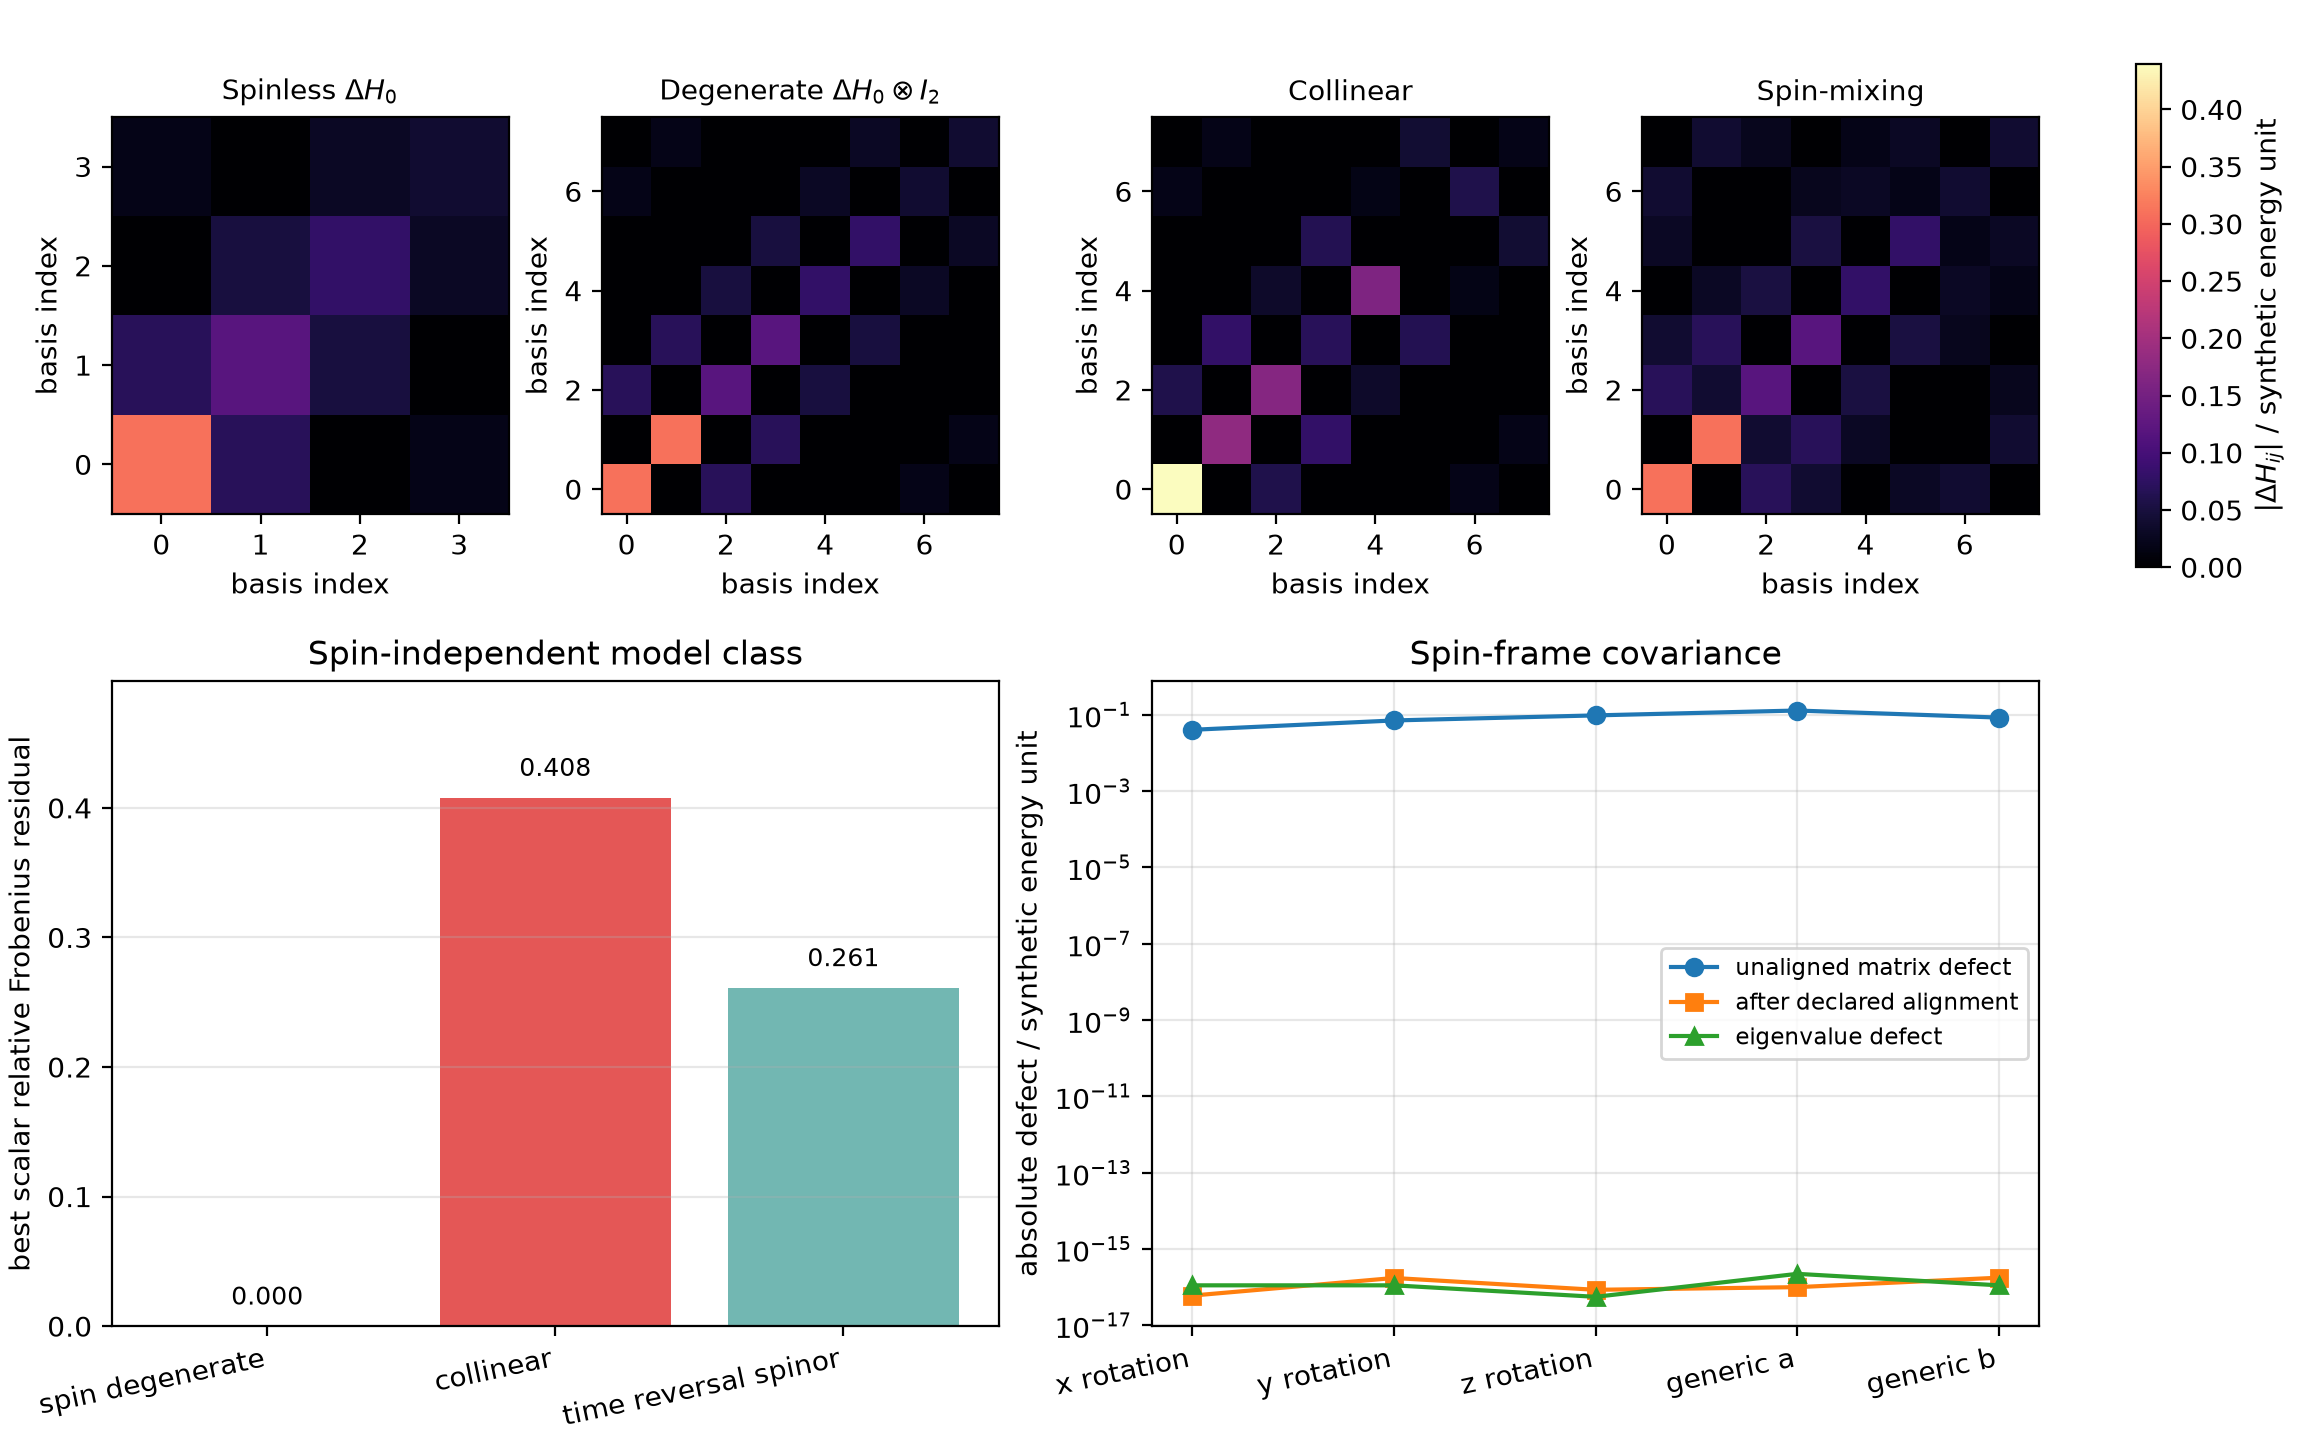
\includegraphics[
    width=\textwidth,
    height=0.82\textheight,
    keepaspectratio
  ]{../../../calculations/research-monograph/impurity-spin-spaces/summary.png}
  \caption{Controlled spin-space embedding benchmark. The upper row shows the
  absolute represented matrices for the spinless, spin-degenerate, collinear,
  and spin-mixing impurity operators in their declared coordinates. The lower
  left compares the optimal spin-independent residual for the three spinful
  classes. The lower right contrasts raw spin-frame coordinate differences
  with aligned matrix and eigenvalue defects. Values at the roundoff floor are
  displayed logarithmically only to distinguish them from finite unaligned
  differences.}
  \label{fig:impurity-spin-space-benchmark}
\end{figure}

\subsection{Warmup 2: One-dimensional matched pristine and defect supercells}

Use the one-dimensional periodic parent developed in Note~5. Let a supercell
contain $N_s$ primitive cells and have length
\begin{equation}
    L=N_sa.
\end{equation}
The reduced supercell crystal momentum is denoted $K$. Let
\begin{align}
    \mathbf H_{b,L}(K)
    &: \mathcal V_{b,L}(K)
    \longrightarrow
    \mathcal V_{b,L}(K),
    \\
    \mathbf H_{d,L}(K)
    &: \mathcal V_{d,L}(K)
    \longrightarrow
    \mathcal V_{d,L}(K)
\end{align}
be matched pristine and defect supercell fibers. Both must use the same
supercell length, boundary phase, discretization or orbital convention, spin
space, units, and energy reference before alignment.

The pristine supercell must first reproduce primitive-cell band folding. For
each $K$, the primitive momenta folded into the supercell fiber are
\begin{equation}
    k_{\alpha}
    =
    K+\frac{2\pi\alpha}{L},
    \qquad
    \alpha=0,\ldots,N_s-1,
\end{equation}
reduced modulo the primitive reciprocal lattice. Define a unitary folding map
\begin{equation}
    \mathbf F_L(K):
    \bigoplus_{\alpha=0}^{N_s-1}
    \mathcal V_b(k_{\alpha})
    \longrightarrow
    \mathcal V_{b,L}(K).
\end{equation}
It should satisfy
\begin{equation}
    \mathbf F_L(K)^\dagger
    \mathbf H_{b,L}(K)
    \mathbf F_L(K)
    =
    \bigoplus_{\alpha=0}^{N_s-1}
    \mathbf H_b(k_{\alpha})
\end{equation}
for an exactly repeated pristine representation, up to the declared ordering
and numerical approximation. This verifies primitive-to-supercell mapping
before a defect is introduced.

The zero-defect control sets
\begin{equation}
    \mathbf H_{d,L}(K)=\mathbf H_{b,L}(K)
\end{equation}
before independent coordinate changes. After gauge, ordering, and energy
alignment, the extracted impurity operator must be zero within the stated
numerical tolerance.

Next introduce a known periodic supercell defect:
\begin{equation}
    \mathbf H_{d,L}^{\mathrm{known}}(K)
    =
    \mathbf H_{b,L}(K)
    +
    \mathbf V_{\mathrm{known},L}(K).
\end{equation}
The planted operator should progress through:
\begin{enumerate}
    \item a one-site scalar shift;
    \item an orbital-dependent onsite shift;
    \item a modified nearest-neighbor hopping;
    \item a finite-range nonlocal defect;
    \item a collinear spin-dependent defect; and
    \item a spin-mixing defect after the spinor warmup is verified.
\end{enumerate}
The doped representation should then be independently transformed by a known
unitary, orbital permutation, supercell translation, and scalar energy shift.
The declared alignment procedure should recover the planted operator in the
pristine reference coordinates.

The one-dimensional supercell warmup should be repeated over increasing
$N_s$. Each finite $L$ represents a periodic defect array. A localized isolated
defect level is represented at finite $L$ by a defect-derived supercell band
$E_{d,\ell}(K;L)$ rather than by one $K$-independent bound-state energy. Its
center, bandwidth, dispersion, and separation from the declared host band edge
should be tracked together with central blocks, exterior blocks, cross
couplings, and localization diagnostics as image separation increases.

\subsubsection{Calculated synthetic verification}

The controlled calculation reuses the accepted periodic one-dimensional
parents: the lowest isolated-band hopping record and the smooth two-band
\texttt{low\_pair} blocks truncated to $|R|\leq4a$. Their exact content
identities, together with the complete input, protocol, result, independent
verifier, report, and figure, are retained under
\path{calculations/research-monograph/impurity-defect-1d/}. All defects and
alignment maps are synthetic and known by construction.

For an $N_s=16$ two-orbital supercell, three reduced supercell momenta give a
largest primitive-folding operator defect of
$9.69\times10^{-15}E_G$ and a largest eigenvalue defect of
$7.77\times10^{-16}E_G$. The folding-map unitarity defect remains below
$1.87\times10^{-14}$. Seven matched controls then plant null, scalar onsite,
orbital onsite, range-one hopping, range-two hopping, collinear-spin, and
spin-mixing operators. The raw defect representation is changed by a
three-cell translation, an orbital swap, orbital rotation and phases, a
site-dependent phase,
a global spin-frame rotation where applicable, and a scalar reference shift of
$0.137E_G$. Metadata prevent direct subtraction. After applying the declared
inverse maps, the largest planted-operator recovery defect is
$1.32\times10^{-15}E_G$; the null recovery defect is
$8.72\times10^{-16}E_G$. Omitting only the scalar-reference correction creates
an exterior false offset of $0.750E_G$ in the spinless controls.

A hierarchy frozen before evaluation selects the scalar onsite, orbital onsite,
range-one, range-two, collinear, and general spinor classes exactly where those
structures were planted. The preceding relative residuals are respectively
$0.474$ for an orbital defect projected into the scalar class, unity for both
nonlocal defects projected into insufficient-range classes, $0.278$ for a
collinear defect projected into the spin-independent class, and $0.184$ for a
spin-mixing defect projected into the collinear class. Six deliberately
incompatible rank, spin, geometry, site, retained-subspace, and
energy-reference cases stop without a nominal residual.

For a fixed Gaussian orbital defect, increasing $N_s$ from 12 to 48 reduces the
lowest defect-band width from $5.95\times10^{-7}E_G$ to the numerical floor.
The center binding changes by $4.76\times10^{-12}E_G$, the two-state bound
count is unchanged, and the lowest-state RMS radius stabilizes near $0.733776a$.
The fixed core operator is unchanged across the sequence; its exterior norm,
$2.07\times10^{-5}E_G$ for the declared radius-$2a$ split, remains separately
reported rather than being inferred from the spectral convergence.

On a separate scalar $N_s=128$ comparison grid, widening fixed-peak and
fixed-integrated Gaussian profiles from $0.5a$ to $8a$ reduces the absolute
lattice--parabolic binding discrepancy from $5.53\times10^{-3}E_G$ to
$2.36\times10^{-5}E_G$ and from $8.84\times10^{-3}E_G$ to
$2.65\times10^{-6}E_G$, respectively. The corresponding broad-profile
fidelities are $0.999977$ and $0.9999975$. This is a trend on one finite,
band-limited comparison grid, not a converged continuum-crossover result.

Two constructed residuals expose the independence of operator and observable
metrics. A rank-one excited-sector residual of norm $0.500E_G$ leaves the
lowest binding and state unchanged to roundoff. A smaller
$9.66\times10^{-3}E_G$ bound--continuum coupling changes the binding by
$2.83\times10^{-3}E_G$ and lowers the state fidelity to $0.8536$. Neither a
large nor a small global operator norm is therefore an observable certificate
without additional spectral information.

Figure~\ref{fig:impurity-defect-1d-benchmark} summarizes these controls. This
is a human-accepted calculated synthetic numerical-verification result within
the bounded exercise. It establishes only software and numerical verification
of the synthetic construction. It is not a silicon
impurity calculation, material effective-mass validation, continuum-limit
proof, or uncertainty quantification.

\begin{figure}[p]
  \centering
  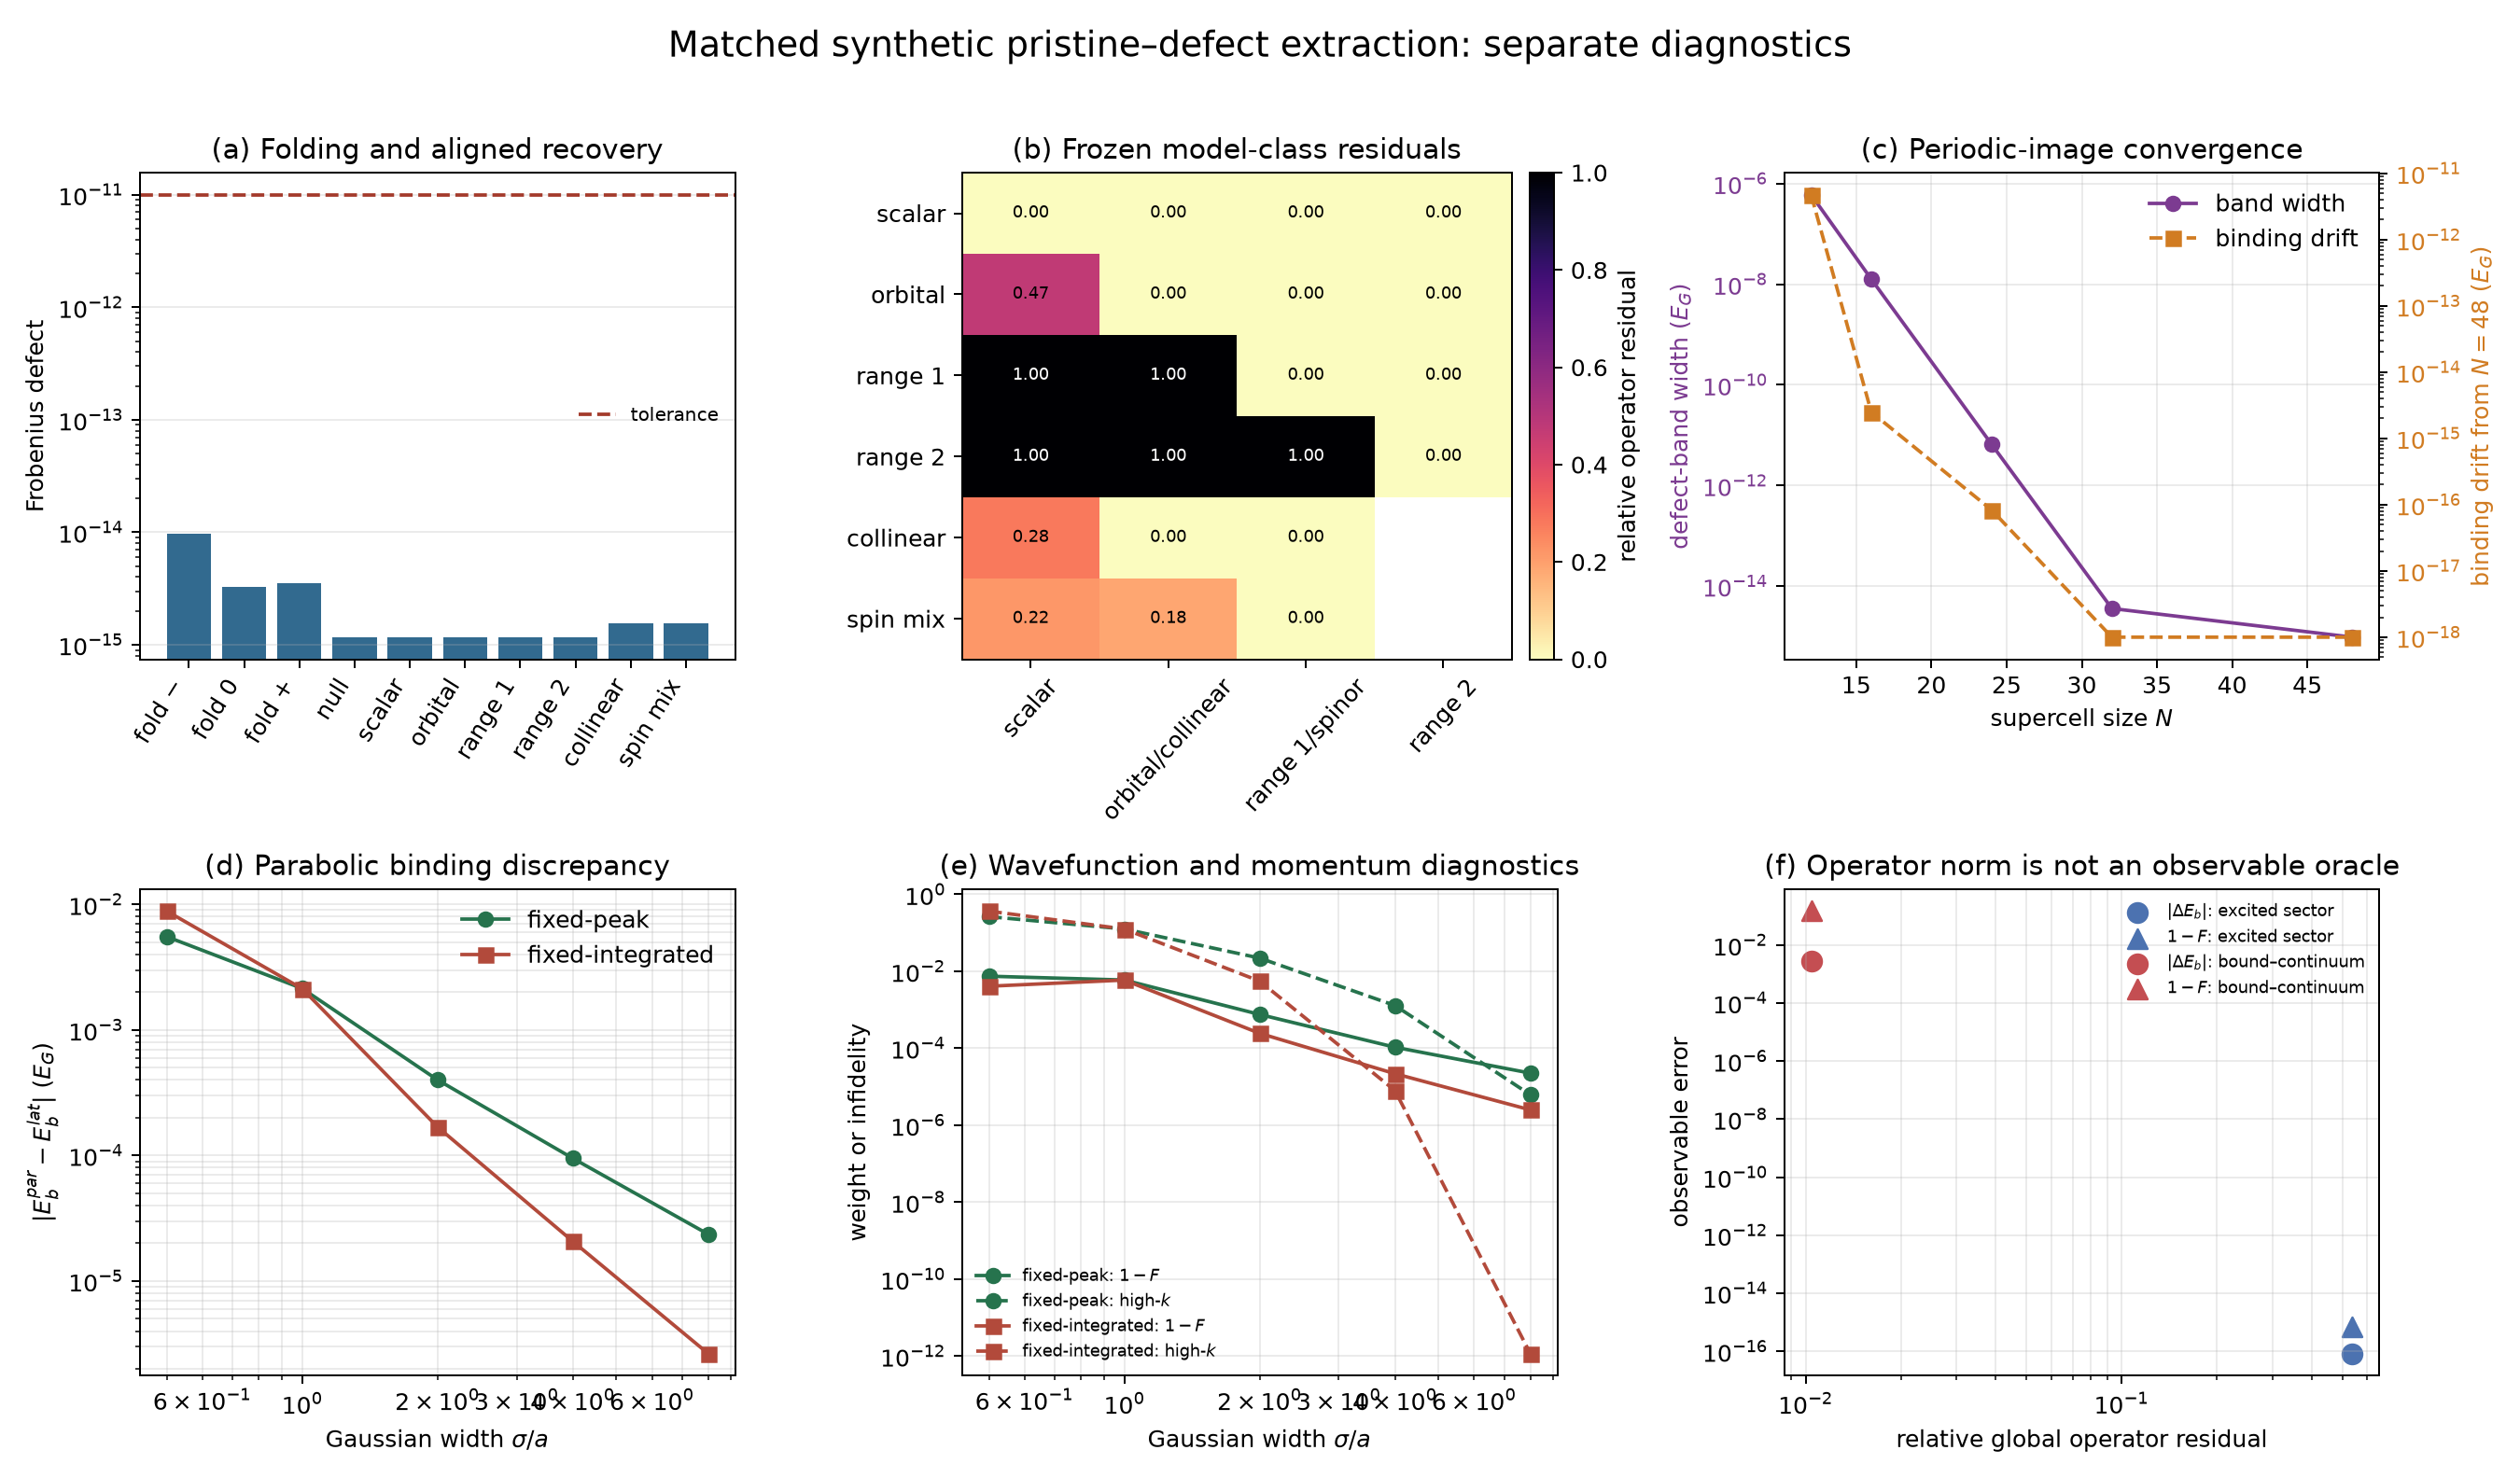
\includegraphics[
    width=\textwidth,
    height=0.82\textheight,
    keepaspectratio
  ]{../../../calculations/research-monograph/impurity-defect-1d/summary.png}
  \caption{Matched one-dimensional pristine--defect benchmark. Panel (a)
  reports primitive-folding and aligned planted-recovery defects against the
  frozen algebraic tolerance. Panel (b) gives classwise relative operator
  residuals for the frozen hierarchy. Panel (c) separates defect-band width
  from binding-center drift over the supercell sequence. Panels (d) and (e)
  retain lattice--parabolic binding, wavefunction, and high-momentum
  diagnostics for fixed-peak and fixed-integrated profile families. Panel (f)
  contrasts global operator residuals with binding and fidelity errors in two
  constructed spectral sectors.}
  \label{fig:impurity-defect-1d-benchmark}
\end{figure}

\subsubsection{Calculated blind-alignment verification}

A separate synthetic inverse problem withholds the authored translation,
orbital, spin-frame, scalar energy shift, and planted defect from the inference
action. The action instead receives the two represented Hamiltonians, an
authored anchor cross-covariance, retained-subspace information, an exterior
energy anchor, and spin labels. A truncated polar factor supplies the inferred
map, and the scalar shift is estimated from the aligned exterior sector before
subtraction. Oracle data enter only in post hoc evaluation. The complete input,
protocol, result, independent verifier, report, and figures are retained under
\path{calculations/research-monograph/impurity-defect-1d-blind-alignment/}.

In the 32-dimensional spinless and 64-dimensional spinor full-rank controls,
the phase-quotiented map defects are $9.68\times10^{-15}$ and
$1.41\times10^{-14}$, while the planted-operator recovery defects are
$5.54\times10^{-15}E_G$ and $9.32\times10^{-15}E_G$. The scalar-shift error is
$5.55\times10^{-17}E_G$ in both cases. Map, energy-reference, extraction,
onsite-model, active-spectrum, and lowest-state errors remain separate.

A 16-of-32-dimensional undercomplete anchor identifies only a compressed
sector. Two admissible unitary completions disagree by $9.92\times10^{-1}E_G$
as full extracted operators, but their compressed disagreement is
$7.73\times10^{-16}E_G$ and their partial maps agree to
$1.08\times10^{-15}$. The unobserved complement is therefore retained as a
gauge freedom rather than assigned a forced map. A controlled unitary anchor
perturbation produces graded downstream errors; at $10^{-2}$ rad the map,
extraction, and active-spectrum defects are respectively $2.78\times10^{-2}$,
$1.62\times10^{-2}E_G$, and $6.81\times10^{-3}E_G$. This is a deterministic
sensitivity scan, not uncertainty quantification.

Ill-conditioned anchors, incompatible retained subspaces, unequal represented
ranks, incompatible spin spaces, and a missing exterior energy anchor return
structured stops without an extracted operator. An independent implementation
reconstructs every retained nominal metric and stopping outcome without
importing the runner. Figure~\ref{fig:impurity-defect-1d-blind-alignment}
summarizes the result. It is a human-accepted synthetic software and numerical
verification result within this bounded exercise, not a material alignment or
uniqueness claim.

\begin{figure}[p]
  \centering
  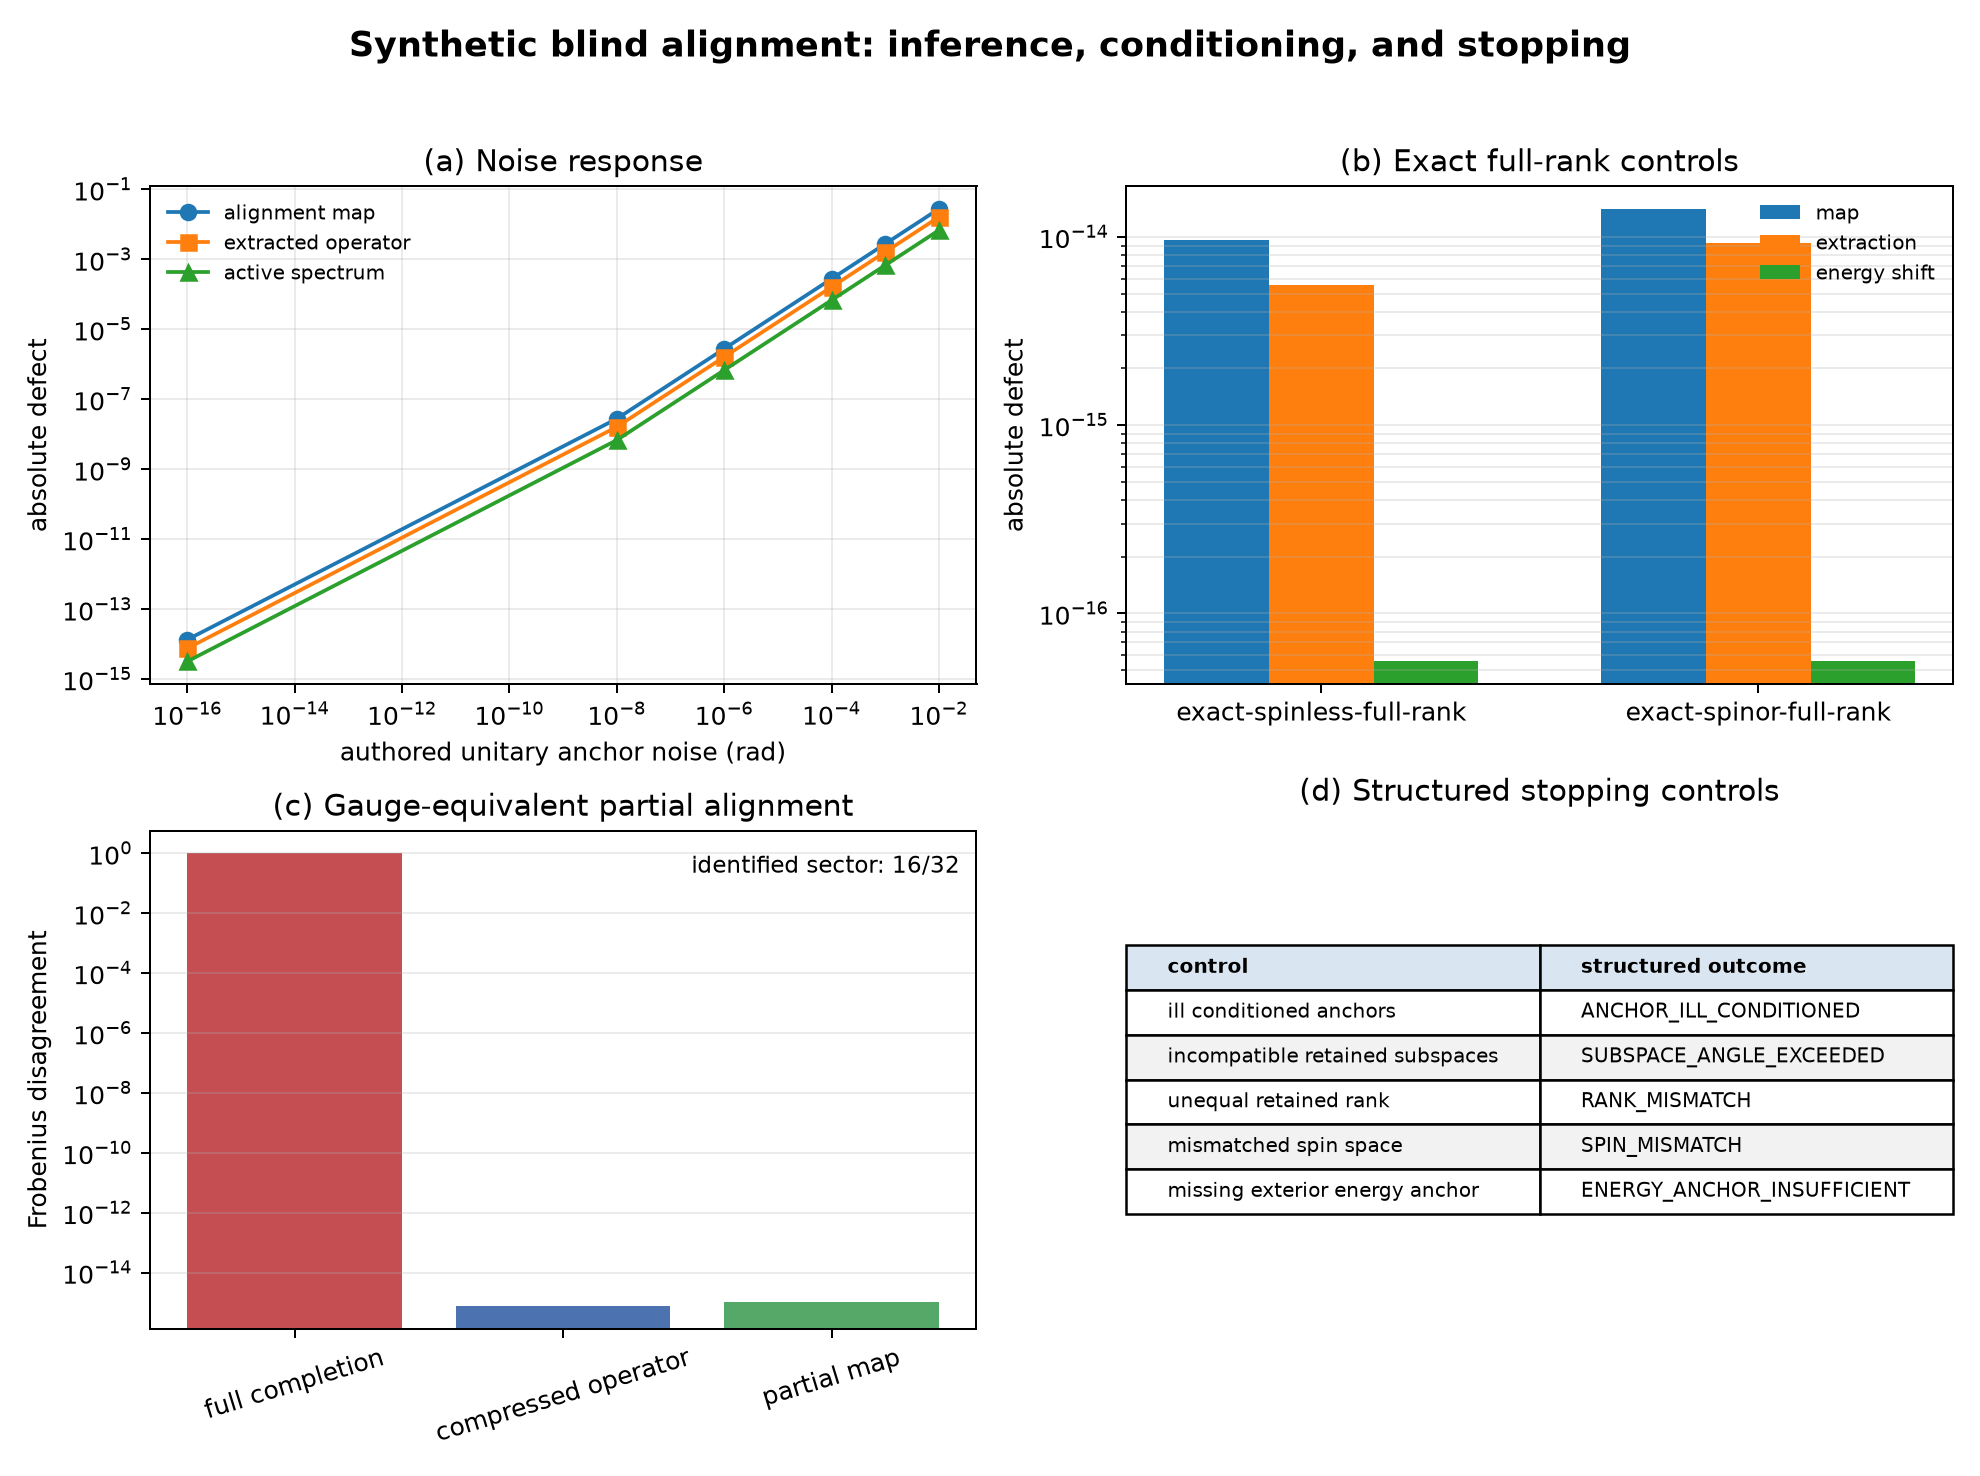
\includegraphics[
    width=\textwidth,
    height=0.78\textheight,
    keepaspectratio
  ]{../../../calculations/research-monograph/impurity-defect-1d-blind-alignment/summary.png}
  \caption{Synthetic blind-alignment benchmark. Panel (a) separates alignment,
  extracted-operator, and active-spectrum responses to controlled unitary
  anchor perturbations. Panel (b) gives the exact full-rank controls. Panel (c)
  contrasts full-completion non-identifiability with agreement in the declared
  compressed sector. Panel (d) lists the five structured stopping controls.}
  \label{fig:impurity-defect-1d-blind-alignment}
\end{figure}

Neighboring diagnostics preserve those five stops while exposing their
boundaries. With fixed additive anchor noise $10^{-10}$, map and extraction
errors grow to $2.64\times10^{-6}$ and $1.22\times10^{-6}E_G$ at condition
number $5.00\times10^5$; the next point, $1.25\times10^6$, stops against the
frozen $10^6$ limit. A one-direction principal-angle sweep passes at $0.34$
rad and stops at $0.36$ rad against the $0.35$-rad rule. Exterior energy-anchor
ranks zero through three stop, whereas rank four recovers the shift to
$2.78\times10^{-17}E_G$. This boundary probe corrected an implementation
defect: energy-anchor rank is now computed from singular values above the
numerical-rank tolerance rather than by comparing a rounded floating-point
trace with an integer threshold.

Unequal ranks remain invalid for full unitary comparison, but an explicitly
declared $32\times31$ partial isometry recovers its common-sector map and zero
operator to $9.92\times10^{-15}$ and $6.58\times10^{-15}E_G$. Because the zero
operator has a 31-dimensional lowest eigenspace, the individual lowest-state
fidelity is left undefined and its eigenspace-projector defect,
$7.28\times10^{-15}$, is reported instead. The spin mismatch similarly remains
invalid directly; an explicit spin lift recovers the common spinor
representation, while the spin-independent restriction residual
$7.97\times10^{-2}E_G$ shows that the planted spin mixing cannot be restricted
losslessly. Figure~\ref{fig:impurity-defect-1d-blind-alignment-debugging}
retains these diagnostics. The cutoffs are synthetic protocol settings rather
than material tolerances.

\begin{figure}[p]
  \centering
  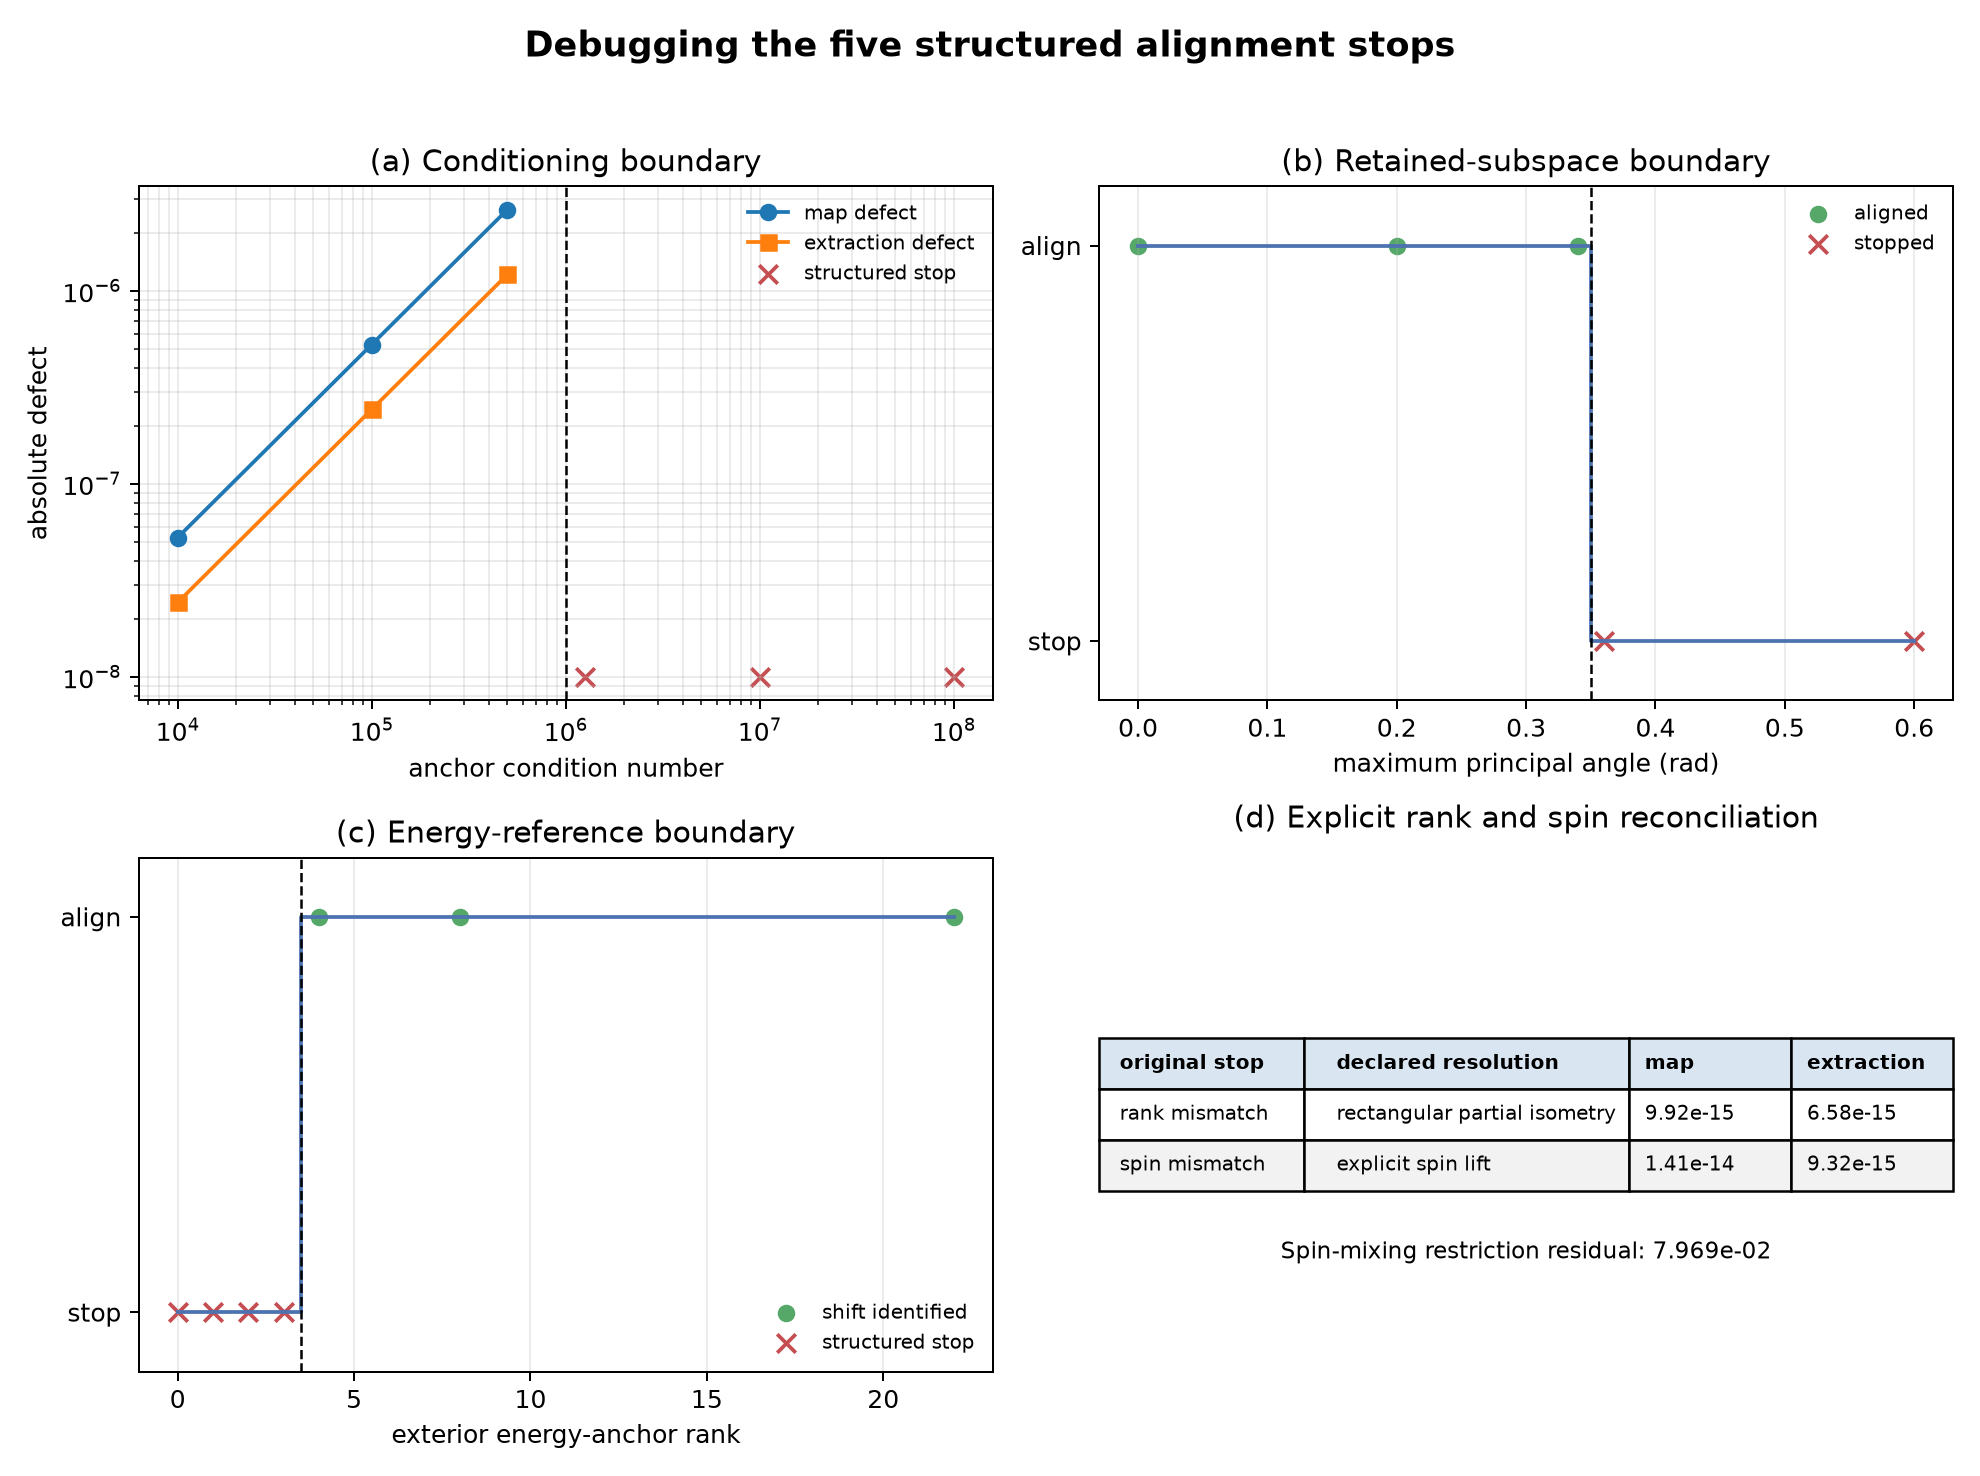
\includegraphics[
    width=\textwidth,
    height=0.78\textheight,
    keepaspectratio
  ]{../../../calculations/research-monograph/impurity-defect-1d-blind-alignment/diagnostics.png}
  \caption{Debugging the five structured stops without weakening them. Panels
  (a)--(c) locate the conditioning, principal-angle, and exterior-energy-anchor
  boundaries. Panel (d) reports explicitly declared common-space resolutions
  for unequal rank and unequal spin space; these do not make the original raw
  comparisons admissible.}
  \label{fig:impurity-defect-1d-blind-alignment-debugging}
\end{figure}

\subsubsection{Calculated independent-route verification}

A second synthetic follow-on compares two implementations after the same
coordinate and energy-reference alignment has been declared. Route A assembles
and subtracts finite-supercell matrices directly in site space. Route B does
not call Route A: it evaluates the primitive $2\times2$ Bloch matrices, builds
the 16-point folding map, and subtracts directly in folded-fiber space. The
commutativity question is whether $F^\dagger V^{(A)}F=V^{(B)}$. Exact source
identities, input, protocol, result, independent verifier, report, and figure
are retained under
\path{calculations/research-monograph/impurity-defect-1d-independent-route/}.

All seven null, local, nonlocal, collinear, and spin-mixing controls commute
within the frozen $10^{-11}$ tolerance. The largest pristine-representation
and route-noncommutativity defects are $9.58\times10^{-15}E_G$ and
$9.61\times10^{-15}E_G$; the largest reconstructed eigenvalue discrepancy is
$1.11\times10^{-15}E_G$. Direct site-space and direct fiber-space planted
recovery remain below $1.56\times10^{-15}E_G$ and
$9.70\times10^{-15}E_G$, respectively. An independent verifier reconstructs
both routes without importing the runner.

Changing only the fiber-route hopping range from $4a$ to $3a$ produces
operator noncommutativity $2.83\times10^{-2}E_G$ even though the reconstructed
physical spectra still agree to $7.77\times10^{-16}E_G$. Thus spectral
agreement does not certify the extracted operator when the pristine parent
partition differs. A 15-fiber domain, nonuniform quadrature weights, and an
unmatched alignment map stop before nominal extraction. All four altered
contracts are paired with explicit compatible constructions: a common
$|R|\leq3$ parent, a common 15-cell/15-fiber domain, the dual
$G^{-1}=W^{-1/2}F^\dagger$ and induced metric for weighted coordinates, and the
relative unitary $R=T_AT_B^\dagger$ between alignment frames. Their route
defects are at most $6.82\times10^{-15}E_G$. The common-range parent still
differs from the nominal parent by $2.83\times10^{-2}E_G$; thus the original
mixed-parent noncommutativity and the three stops remain valid guards because
common contracts must be declared rather than inferred silently.
Figure~\ref{fig:impurity-defect-1d-independent-route} summarizes the comparison.
This is a human-accepted bounded synthetic software and numerical-verification
result, not material or continuum validation.

\begin{figure}[p]
  \centering
  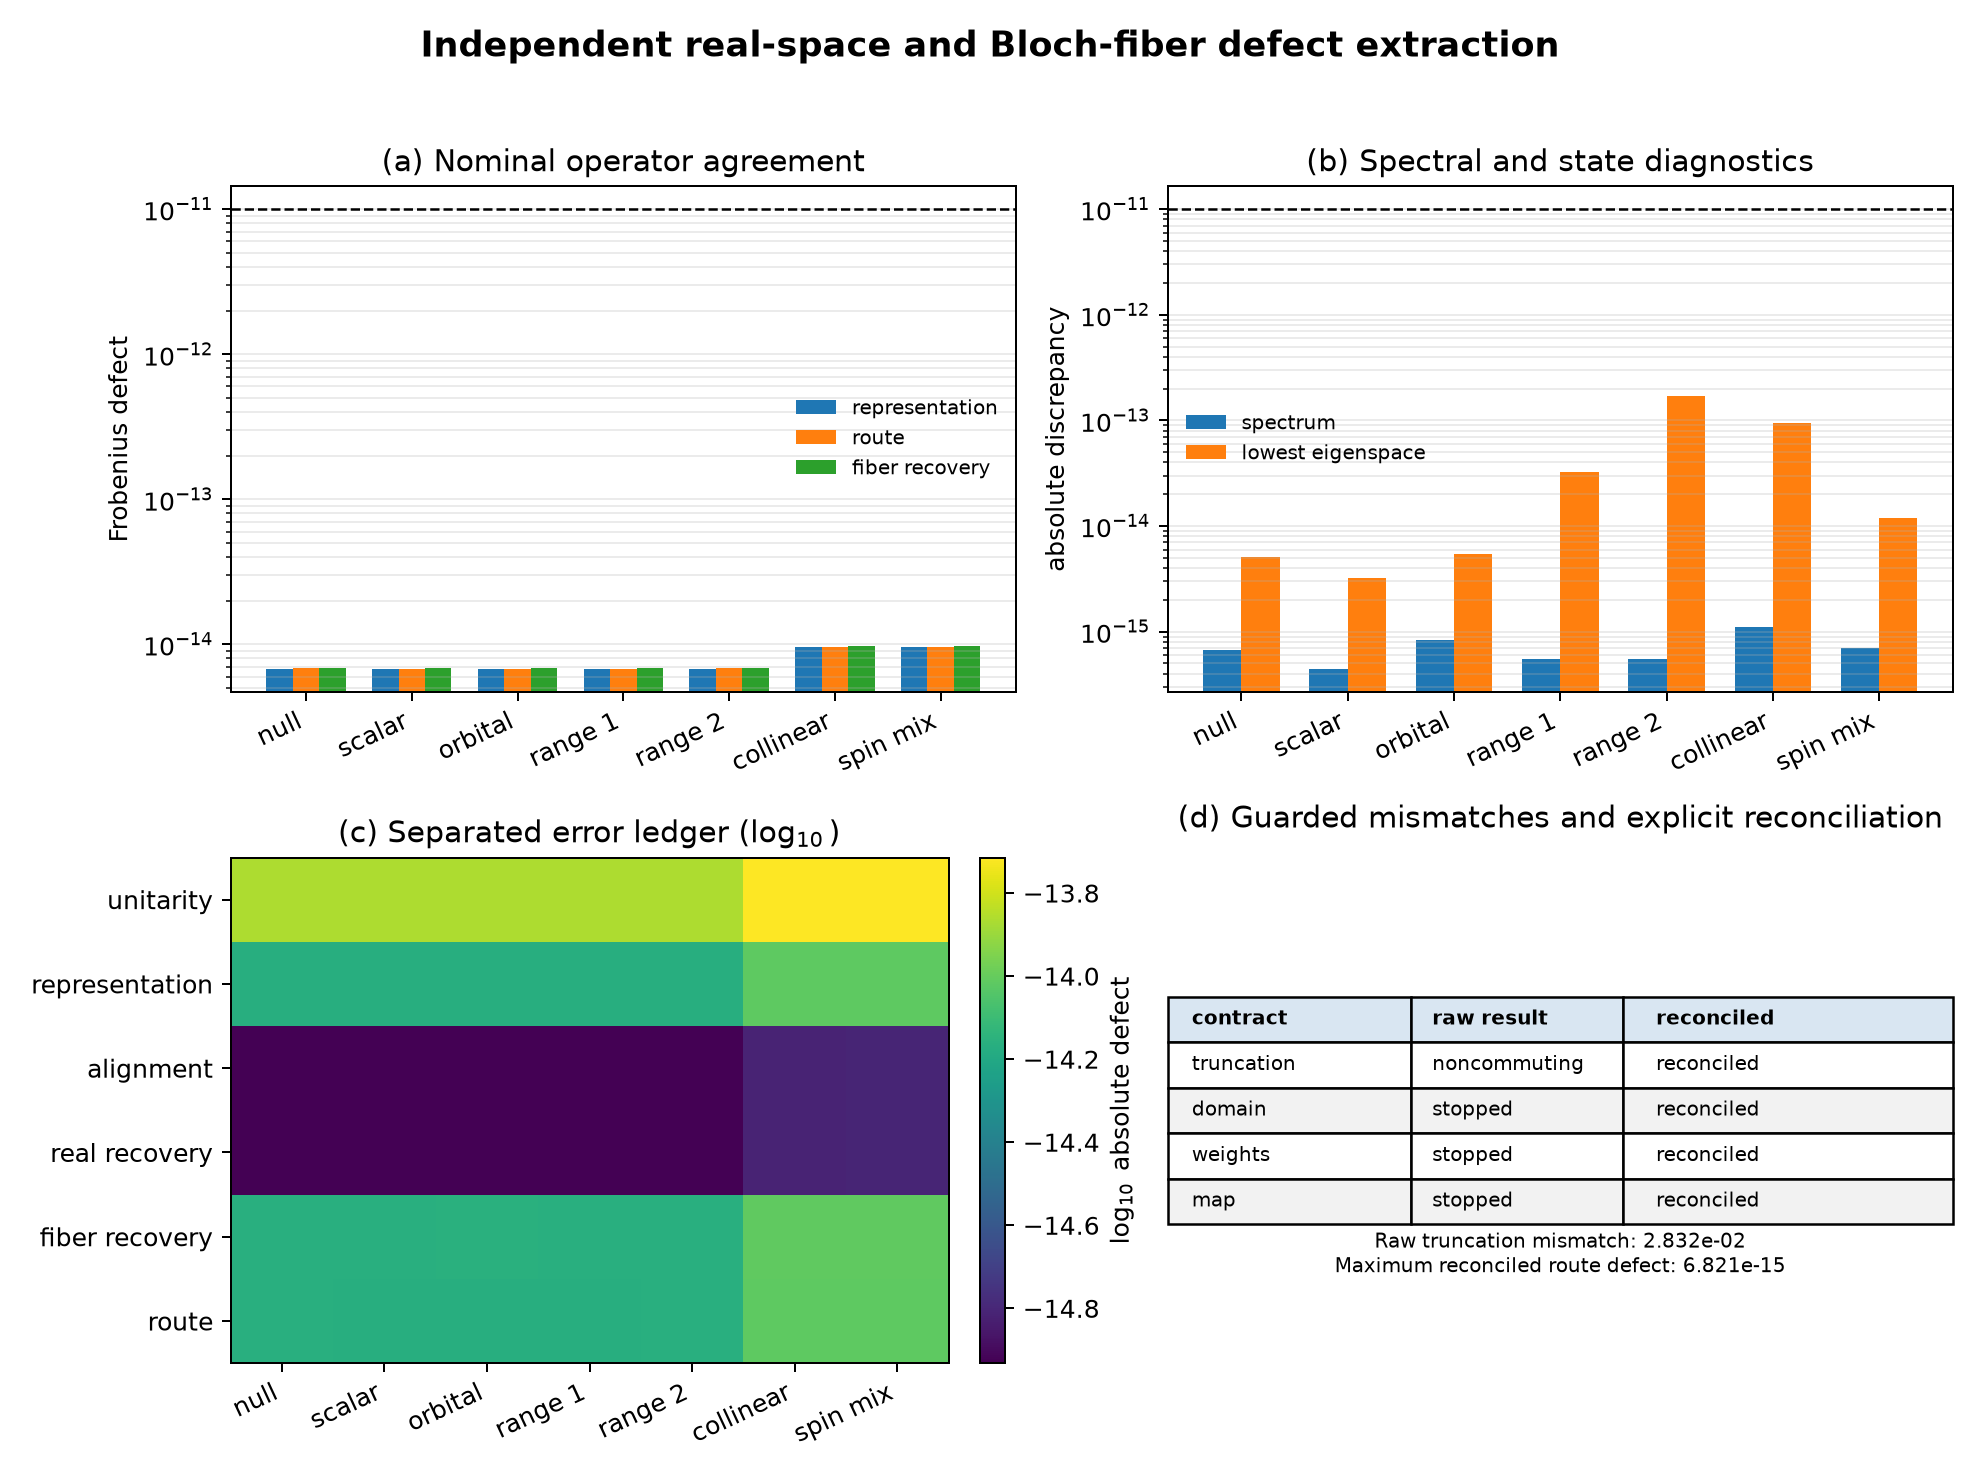
\includegraphics[
    width=\textwidth,
    height=0.78\textheight,
    keepaspectratio
  ]{../../../calculations/research-monograph/impurity-defect-1d-independent-route/summary.png}
  \caption{Independent-route synthetic benchmark. Panel (a) compares
  representation, route, and planted-recovery errors. Panel (b) retains
  spectral and lowest-eigenspace discrepancies separately. Panel (c) shows the
  complete separated error ledger. Panel (d) distinguishes fail-closed
  mismatch outcomes from explicit common-parent, common-domain, dual-map, and
  relative-unitary reconciliations.}
  \label{fig:impurity-defect-1d-independent-route}
\end{figure}

\subsubsection{One-dimensional follow-on sequence}

The accepted known-map exercise remains the fixed ground-truth baseline. The
first and second follow-ons are human accepted; the sequence remains:
\begin{enumerate}
    \item infer hidden translation, orbital, spin-frame, and scalar-reference
          maps from explicitly declared overlap or anchor data, with gauge
          equivalence, degeneracies, principal-angle stops, and noise treated as
          part of the alignment contract;
    \item compare real-space extraction with an independently implemented
          Bloch-fiber or folding route and test their commutativity after
          alignment;
    \item add an analytically solvable finite-rank defect whose bound-state
          energy and state follow from an independent resolvent equation;
    \item refine continuum spacing, domain length, supercell size, and defect
          width independently before proposing a continuum crossover; and
    \item position the definitions and observed failure modes against verified
          primary literature before making a novelty claim.
\end{enumerate}
The first item is the accepted blind-alignment result reported above, and the
second is the accepted bounded independent-route result. Items three through five
remain proposed follow-on experiments rather than extensions of the accepted
result, and none is an active material calculation. Keeping the alignment
inverse problem separate preserves attribution: failure to infer the map is not
confused with failure of subtraction after a correct map is supplied.

\subsection{Warmup 3: Two-dimensional matched pristine and defect supercells}

Use the separable and coupled two-dimensional parents developed in Note~6. Let
the supercell contain $N_x\times N_y$ primitive cells with lattice vectors
\begin{equation}
    \mathbf L_1=N_x\mathbf a_1,
    \qquad
    \mathbf L_2=N_y\mathbf a_2.
\end{equation}
The matched pristine and defect fibers are
\begin{align}
    \mathbf H_{b,\mathbf L}(\mathbf K),
    \qquad
    \mathbf H_{d,\mathbf L}(\mathbf K),
\end{align}
with $\mathbf K$ in the reduced supercell Brillouin zone.

The pristine control must reproduce two-dimensional folding from the primitive
mesh into each supercell fiber. In the separable limit, the supercell
construction should also reproduce products and sums of the verified
one-dimensional results. Degenerate folded clusters must be compared through
their complete projectors rather than through arbitrary eigenvector labels.

The first planted defect should be a scalar onsite or localized multiplication
term at a declared supercell site. Later stages should add:
\begin{enumerate}
    \item direction-dependent hopping changes;
    \item a finite-range nonlocal defect;
    \item orbital or composite-band mixing;
    \item anisotropic spatial profiles;
    \item spin-dependent and spin-mixing terms; and
    \item a defect in the nonseparable two-dimensional parent.
\end{enumerate}
Independent point-group-related placements should produce aligned operators
related by the corresponding lattice symmetry. A failure of this covariance
should be attributed among site mapping, supercell origin, gauge, degeneracy
handling, and boundary phases before the defect model is interpreted.

The finite-size study must vary both area and shape. Square sequences probe
increasing image separation under preserved symmetry, while rectangular
sequences test anisotropic image interactions and alignment conventions. One
apparently converged square supercell is not sufficient evidence for an
isolated two-dimensional defect.

\subsection{Control 4: Energy-reference, gauge, ordering, and geometry stress tests}

For a known aligned defect, construct a raw candidate representation
\begin{equation}
    \widetilde{\mathbf H}_{d}
    =
    \mathbf G
    \left(
        \mathbf H_b+\mathbf V_{\mathrm{known}}
    \right)
    \mathbf G^\dagger
    +
    c\mathbf I,
\end{equation}
where $\mathbf G$ is a known admissible coordinate transformation and $c$ is a
known scalar shift. The transformation sequence should include:
\begin{enumerate}
    \item orbital phases;
    \item orbital and site permutations;
    \item unitary rotations within degenerate subspaces;
    \item primitive or supercell translations;
    \item admissible point-group transformations;
    \item changes of localized gauge; and
    \item a scalar energy-reference offset.
\end{enumerate}
After applying the inverse declared alignment and energy-reference procedure,
the extracted operator should equal $\mathbf V_{\mathrm{known}}$ within the
stated representation error.

The tests should also contain deliberately incompatible cases: unequal retained
rank, mismatched spin space, incorrect supercell shape, lost site
correspondence, or large principal angles between retained subspaces. These
cases should stop the comparison. They should not be forced into a unitary fit
merely because two final matrices can be made equal in dimension.

The energy-reference test is particularly important. Without correction,
$c\mathbf I$ appears as a spatially extended false impurity term. The alignment
procedure must remove only the declared reference offset and must not subtract
a genuine localized onsite component.

\subsection{Control 5: Supercell-size and shape convergence}

Let $\Delta\mathbf H_L$ denote an aligned impurity operator for supercell size
or shape label $L$. Define a projector $\mathbf P_r$ onto a declared region
within distance $r$ of the defect and
\begin{equation}
    \mathbf Q_r=\mathbf I-\mathbf P_r.
\end{equation}
Complementary diagnostics include
\begin{align}
    \varepsilon_{\mathrm{core}}(r;L,L')
    &=
    \left\lVert
        \mathbf P_r
        \left(
            \Delta\mathbf H_L-
            \Delta\mathbf H_{L'}
        \right)
        \mathbf P_r
    \right\rVert_{\mathrm F},
    \\
    \varepsilon_{\mathrm{ext}}(r;L)
    &=
    \left\lVert
        \mathbf Q_r
        \Delta\mathbf H_L
        \mathbf Q_r
    \right\rVert_{\mathrm F},
    \\
    \varepsilon_{\mathrm{cross}}(r;L)
    &=
    \left(
        \left\lVert
            \mathbf P_r
            \Delta\mathbf H_L
            \mathbf Q_r
        \right\rVert_{\mathrm F}^2
        +
        \left\lVert
            \mathbf Q_r
            \Delta\mathbf H_L
            \mathbf P_r
        \right\rVert_{\mathrm F}^2
    \right)^{1/2}.
\end{align}
The comparison between different supercells requires an explicit embedding or
restriction to common site and orbital coordinates. The notation above assumes
that this identification has already been performed.

A global Frobenius norm can scale with represented volume or the number of
repeated image contributions. It must not replace local, exterior, and
cross-coupling diagnostics. At finite supercell size, defect-derived energies
must be tracked as functions of supercell momentum. Their bandwidth and
$\mathbf K$ dependence diagnose image coupling and should not be collapsed into
a single nominal bound-state energy. Wavefunction localization and
symmetry-resolved blocks should be tracked independently over the same size and
shape sequence.

\subsection{Control 6: Recovery of known model classes}

Let the planted impurity belong exactly to a declared class
$\mathcal M^{(m_0)}$. Fit the ordered hierarchy
\begin{equation}
    \mathcal M^{(0)},
    \mathcal M^{(1)},
    \ldots
\end{equation}
to the extracted operator. The experiment should verify that:
\begin{enumerate}
    \item a scalar onsite class recovers a scalar onsite defect;
    \item an orbital-dependent class is required for orbital splitting;
    \item an onsite class fails for a planted hopping correction;
    \item a local class leaves a nonzero residual for a planted nonlocal
          operator;
    \item a spin-independent class fails for spin splitting or mixing; and
    \item the first class containing the planted structure can recover it
          within the independently established extraction error.
\end{enumerate}
The failure of a simpler class is a desired outcome when the planted defect lies
outside it. This test determines whether the minimum operator separation acts
as an expressiveness diagnostic rather than merely as an optimization score.

The model hierarchy, parameter bounds, weighting, and stopping rule must be
frozen before the outcomes are inspected. An unnecessarily richer class may
fit the planted operator but does not demonstrate that the selection rule can
identify the least adequate class.

\subsection{Control 7: Smoothness-to-continuum crossover}

Introduce a defect profile with tunable width $\sigma$. One fixed-peak family
is
\begin{equation}
    V_{\sigma}^{(\mathrm{peak})}(\mathbf r)
    =
    V_c
    \exp\left(
        -\frac{\lVert\mathbf r\rVert^2}{2\sigma^2}
    \right).
\end{equation}
Its integrated strength changes with $\sigma$. A separate fixed-integrated
family in spatial dimension $D$ is
\begin{equation}
    V_{\sigma}^{(\mathrm{int})}(\mathbf r)
    =
    \frac{g}{(2\pi\sigma^2)^{D/2}}
    \exp\left(
        -\frac{\lVert\mathbf r\rVert^2}{2\sigma^2}
    \right),
\end{equation}
where $g$ is held fixed. The two protocols answer different questions and must
not be mixed in one convergence sequence. Each profile is periodized only
through a supercell large enough for image effects to be measured separately.

The ratio
\begin{equation}
    \rho=\frac{\sigma}{a}
\end{equation}
is one control, not a complete continuum criterion. The study must also record
the defect strength relative to the relevant bandwidth or gap, the bound-state
or envelope length relative to $a$ and the supercell, the retained-band and
valley separations, and the lattice and continuum discretizations. Frozen
sequences should range from atomically sharp profiles $\rho=O(1)$ to slowly
varying profiles $\rho\gg1$ under both normalization protocols.

For each $\rho$, compare:
\begin{enumerate}
    \item the exact represented lattice defect;
    \item a local lattice model;
    \item a finite-range nonlocal lattice model;
    \item a single-band effective-mass model where admissible; and
    \item multiband or multivalley continuum classes when the retained parent
          requires them.
\end{enumerate}
The study should measure operator residuals, band or valley mixing, bound-state
energies, subspace fidelity, exterior residuals, and cross couplings. Expected
improvement with increasing $\rho$ is a hypothesis to test, not a result to
assert in advance.

A proposed crossover radius or smoothness threshold is meaningful only when
both exterior and cross-coupling criteria pass and remain stable under lattice,
continuum-discretization, and supercell refinement. If no tested scale passes,
the correct outcome is no established continuum crossover over the tested
domain.

\subsection{Control 8: Operator error versus bound-state error}

For a donor-like state below a declared conduction threshold, one possible
binding convention is
\begin{equation}
    E_b
    =
    E_{\mathrm{edge}}-E_{\mathrm{defect}}>0.
\end{equation}
An acceptor-like branch requires its own signed convention relative to the
aligned valence threshold. The parent and model must use the same declared
band-edge or continuum reference. At finite supercell size, both the defect
level and the relevant edge may depend on supercell momentum, so the comparison
must retain that dependence or state the rule used to extract an isolated-limit
quantity.

For every planted or fitted model, retain separately
\begin{align}
    \varepsilon_H
    &=
    \left\lVert
        \Delta\mathbf H_{
        \mathrm{parent}}
        -
        \Delta\mathbf H_{
        \mathrm{model}}
    \right\rVert_{
    \mathrm F},
    \\
    \Delta E_b
    &=
    E_{b,\mathrm{model}}
    -
    E_{b,\mathrm{parent}},
    \\
    F
    &=
    \left|
        \left\langle
            \psi_{b,\mathrm{parent}}
            \mid
            \psi_{b,\mathrm{model}}
        \right\rangle
    \right|^2
\end{align}
when individual normalized bound states are isolated, aligned, and present in
both models. Before matching states, report the number of in-gap or bound states
under the declared threshold convention. If the parent and model have unequal
counts, the mismatch is itself a failed diagnostic and no arbitrary one-to-one
fidelity should be forced. Degenerate or nearly degenerate clusters of equal
rank require a projector or principal-angle fidelity instead of an arbitrary
state overlap; unequal-rank clusters must retain both the rank mismatch and an
appropriately defined subspace discrepancy.

The one-dimensional synthetic exercise above realizes both contrasting cases:
accurate binding with a large excited-sector operator residual, and a small
global residual with a significant bound-state change. They verify the metric
separation for that constructed finite model only; corresponding material
behavior remains untested.

\subsection{Control 9: Null, covariance, and stopping conditions}

Every stage should include three outcomes:
\begin{description}
    \item[Null control.] With no planted defect, the aligned difference should
      vanish within the established representation and alignment errors.
    \item[Covariance control.] Under an admissible coordinate change, the
      abstract impurity operator should be unchanged and its matrix should
      transform by the declared conjugation rule.
    \item[Stopping control.] Incompatible rank, spin, geometry, subspace, or
      energy-reference data should prevent interpretation rather than produce a
      nominal residual.
\end{description}
These controls should be evaluated before any fitted model is called an
impurity potential or effective-mass representation.

\section{Required warmup order}

The proposed sequence is:
\begin{enumerate}
    \item verify the spinless-to-spinful embedding and Frobenius normalization;
    \item verify primitive-to-pristine-supercell folding;
    \item pass the zero-defect null extraction;
    \item recover known one-dimensional planted defects under gauge and energy
          scrambling;
    \item establish one-dimensional supercell-size convergence;
    \item recover the declared one-dimensional model-class hierarchy;
    \item scan one-dimensional defect smoothness toward a continuum regime;
    \item reproduce the same controls in the separable two-dimensional parent;
    \item introduce anisotropy and nonseparable two-dimensional coupling;
    \item introduce collinear and spin-mixing two-dimensional defects;
    \item compare operator, bound-state, and subspace metrics; and
    \item only then transfer the verified procedures to the matched
          pristine--doped silicon program.
\end{enumerate}
The two-dimensional extraction should not be interpreted until the
one-dimensional procedure recovers a known planted defect under alignment
scrambling and supercell refinement. Likewise, first-principles execution would
not be authorized or scientifically validated merely because the warmups pass.
The first item, items two through seven, and the bounded one-dimensional metric
comparison in item eleven now have human-accepted calculated synthetic evidence.
The blind-alignment and independent-route sequence, the two-dimensional stages,
and material transfer remain proposed work.

\section{Remaining warmup plot placeholder}

The remaining placeholder is two-dimensional covariance: display extracted
defect blocks for symmetry-related placements after alignment, together with
the two-dimensional folding, null, supercell-shape, anisotropy, and metric
controls. The completed one-dimensional Figure~\ref{fig:impurity-defect-1d-benchmark}
replaces the previous one-dimensional placeholders. Every future plot should
identify the parent model, supercell, boundary condition, retained space, spin
convention, planted defect, alignment map, energy reference, model class,
normalization, and evidentiary status. A plot placeholder is not a calculated
result.

\section{Research questions}

The resulting program is organized by four questions.

First, which retained subspace and localized representation preserve the
declared pristine-silicon parent observables while remaining stable under
changes in numerical resolution and gauge?

Second, what is the least complex constrained lattice-model class that
satisfies both spectral and operator-level tolerances for the pristine host?

Third, which unitary identifications make pristine and doped retained operators
comparable, and how sensitive is the aligned impurity operator to admissible
choices of gauge, geometry, and energy reference?

Fourth, at what spatial scale, and within which anisotropic or multivalley model
class, can the aligned phosphorus or boron impurity operator be replaced by an
effective-mass description without losing the declared bound-state and operator
observables?

These questions place the continuum approximation at the end of the reduction
chain rather than assuming it at the outset. The aligned impurity operator is
the object extracted from first principles. A local screened potential, a
nonlocal lattice operator, and a multivalley effective-mass model are competing
admissible representations whose adequacy must be established by comparison.
